\section{Email Service}
\label{sec:email}


\subsection{Design}
Email service\citep{rfc5322} allows users to communicate with each other based on texts. In BT Network, it is set up using \texttt{exim4} package on Laptop 3 (BT003).

\subsection{Implementation}
On Laptop 3 (BT003), the package \texttt{exim4} is installed and configured. Important steps in the configuration are shown in \ref{fig:email-configure}.

\begin{lstlisting}
apt-get install exim4
dpkg-reconfigure exim4-config
\end{lstlisting}

\begin{figure*}[ht!]
    \centering
    \begin{subfigure}[b]{\textwidth}
        \centering
        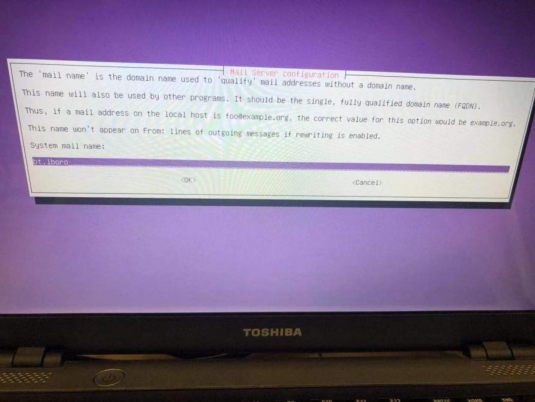
\includegraphics[width=\linewidth]{email-configure-1}
        \caption{Setting Up Mail Name.}
    \end{subfigure}
    ~
    \begin{subfigure}[b]{\textwidth}
        \centering
        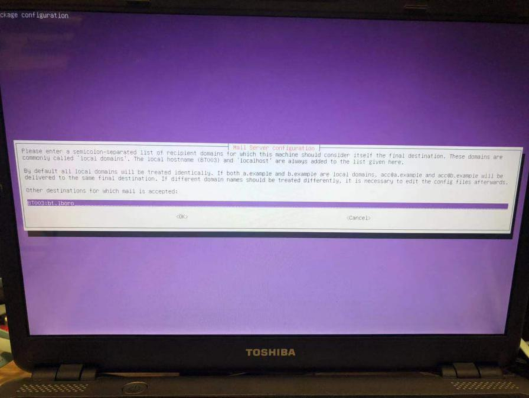
\includegraphics[width=\linewidth]{email-configure-2}
        \caption{Setting Up Domain Name.}
    \end{subfigure}
    \caption{Important Configuration Steps for \texttt{exim4}.}
    \label{fig:email-configure}
\end{figure*}

The full configuration of Email service is detailed in Appendix \ref{app:email}.

\subsection{Evaluation}

For evaluation, the following command are used to send a mail to DT Network. 

\begin{lstlisting}
echo "mua." | sendmail -v mail@dt3.lboro
\end{lstlisting}

The mail can be seen arriving the destination in Figure \ref{fig:email-arrival}.

\begin{figure*}[ht!]
    \centering
    \begin{subfigure}[b]{\textwidth}
        \centering
        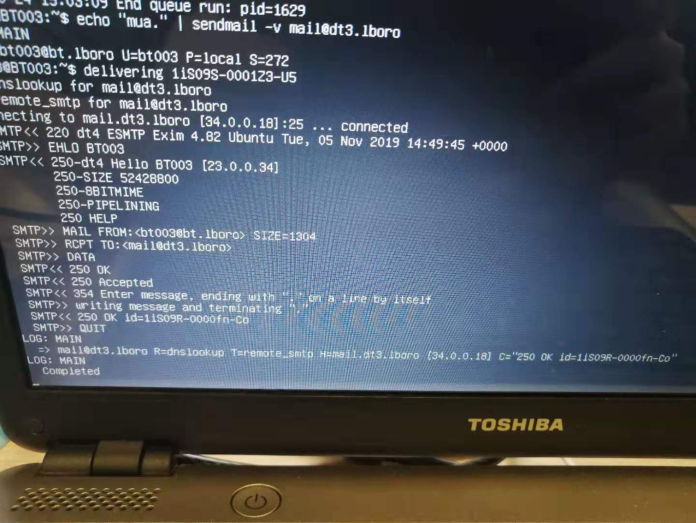
\includegraphics[width=\linewidth]{email-arrival-1}
        \caption{SMTP Sucess Message Is Returned from DT Network on Laptop 3 (BT003).}
    \end{subfigure}
    ~
    \begin{subfigure}[b]{\textwidth}
        \centering
        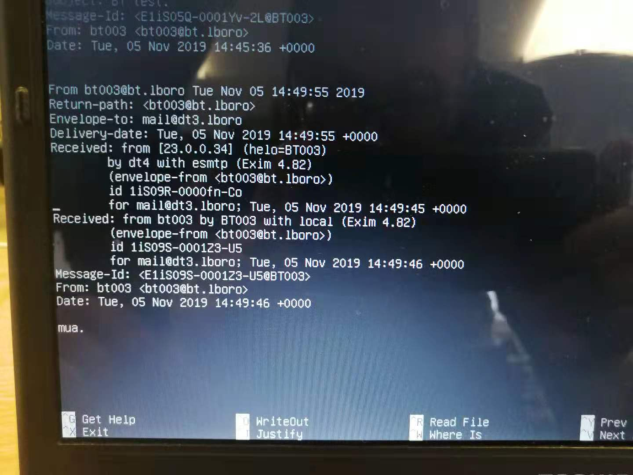
\includegraphics[width=\linewidth]{email-arrival-2}
        \caption{Email Is Received on DT Network's Side.}
    \end{subfigure}
    \caption{Email Can Be Seen Arrived on Both Sides.}
    \label{fig:email-arrival}
\end{figure*}

\subsection{Commentary}

\subsubsection{Problem: Setting Up Domain Name}
At the very beginning, when we were configurating \texttt{exim4}, we just skipped the step and forgot to set up the domain name. 
Later, we found that the mail cannot be sent to other groups. 
The domain name is reset as \texttt{bt.lboro} to solve the problem.

% \subsubsection{Problem: Sending Email}
% After the corrected the domain name, the mail still could not be sent but we could receive the mail from other groups. 
% Finally, through tried for many times we found that the command cannot be written inside the mail which means we must exit at first.










